\section{CNN Seq2seq Model}
\label{sec:cnn}

In this section, we describe the convolutional sequence to sequence (CNN seq2seq) model

\begin{figure}[th]
    \centering
    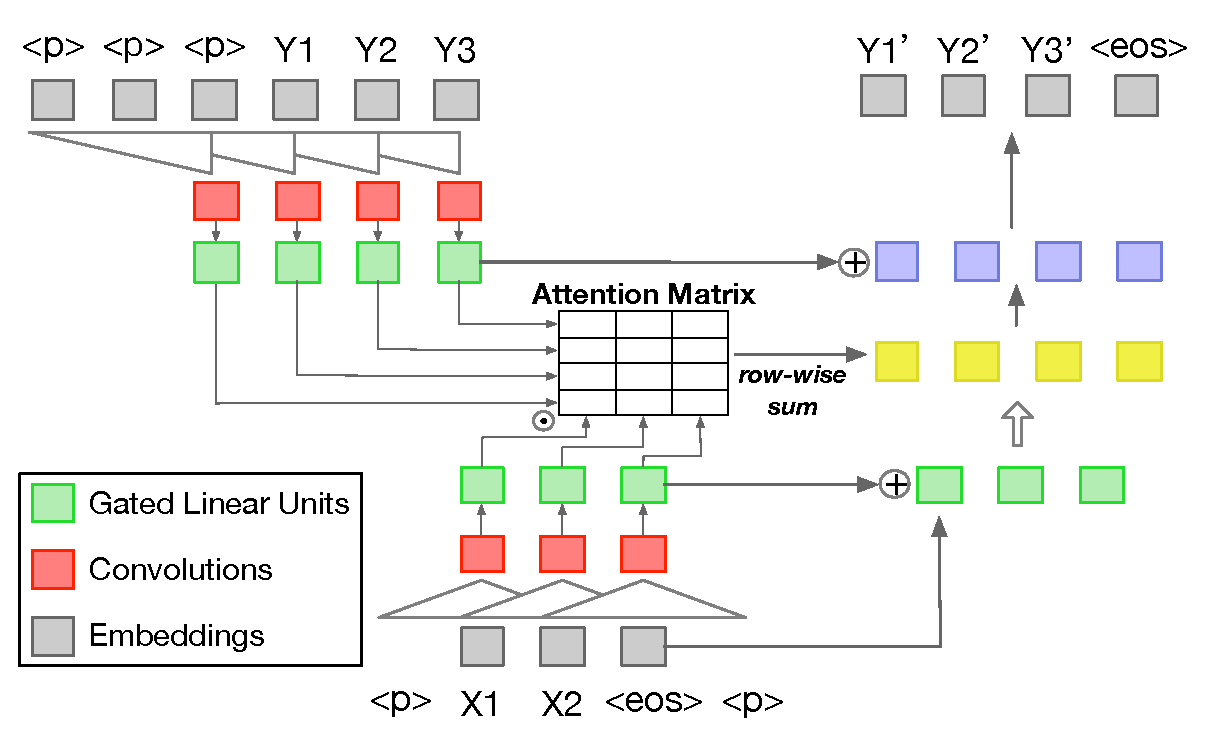
\includegraphics[width=1.0\columnwidth]{cnn}
    \caption{Convolutional seq2seq model. }
    \label{fig:basicModel}
\end{figure}

The CNN seq2seq model includes multi-layer convolutional seq2seq networks \cite{gehring2017convs2s} and attention mechanism \footnote{\url{https://github.com/facebookresearch/fairseq-py}}
(\figref{fig:basicModel}).

In CNN seq2seq models, given the input elements $\textbf{x} = (x_{1},x_{2},...,x_{m})$ and 
output elements $\textbf{y} = (y_{1}, y_{2},..., y_{n})$ ($m>n$),
we obtain the input representations  $\mathbf{X} = (X_1,...,X_m)$ 
and output representations $\mathbf{Y}=(Y_1,...,Y_n)$ by combining
word embeddings and their corresponding position embeddings vectors. 
$\mathbf { z } ^ { l } = \left( z _ { 1 } ^ { l } , \ldots , z _ { m } ^ { l } \right)$ and $\mathbf { h } ^ { l } = \left( h _ { 1 } ^ { l } , \ldots , h _ { n } ^ { l } \right)$ 
are convolutional output of the encoder and decoder in the $l$-th layer.
We use GLU \cite{DauphinFAG17} and residual connections \cite{HeZRS16} after convolution 
in each layer to ensure that the sufficient and effective information is transmitted layer by layer.  
\begin{equation}
\small
    h _ { i } ^ { l } = GLU \left( W ^ { l } \left[ h _ {i-k/2 } ^ { l - 1 } , \ldots , h _ { i+k/2 } ^ { l - 1 } \right] + b _ { w } ^ { l } \right) + h _ { i } ^ { l - 1 }
\end{equation} 
where \textit{k} is kernel width.
We compute the probability
distribution of generating the next elements $y_{i+1}$
based on the current state and transform the top
decoder output $h_{i}^{l}$ via softmax:
\begin{equation}
\small
    p \left( y _ { i + 1 } | y _ { 1 } , \ldots , y _ { i } , \mathbf { x } \right) = \operatorname { softmax } \left( W _ { o } h _ { i } ^ { L } + b _ { o } \right) \in \mathbb { R } ^ { T }
\end{equation}

For each decoder layer, 
we combine the current decoder state $h_{i}$
with an embedding of the previous target element via $Y_{i}$:
\begin{equation}
\small
    d _ { i } ^ { l } = W _ { d } ^ { l } h _ { i } ^ { l } + b _ { d } ^ { l } + Y _ { i }
\end{equation}

The conditional input to the current 
decoder layer is a weighted sum of both encoder states and input element representations.
\begin{equation}\label{eq:a}
\small
    a _ { i j } ^ { l } = \frac { \exp \left( d _ { i } ^ { l } \cdot z _ { j } ^ { u } \right) } { \sum _ { t = 1 } ^ { m } \exp \left( d _ { i } ^ { l } \cdot z _ { t } ^ { u } \right) }
\end{equation}
\begin{equation}\label{eq:c}
\small
    c _ { i } ^ { l } = \sum _ { j = 1 } ^ { m } a _ { i j } ^ { l } \left( z _ { j } ^ { u } + X_j \right)
\end{equation}
%where $z_{j}^{u}$ is the encoder output of last layer $u$.  
where $u$ is the last layer of encoder.  
Finally, $c _ { i } ^ { l }$ is added to $h_{i}^{l}$ as the input for the next decoder layer.

